\documentclass{article}
% 15 cards, 2.5in x 2in, in a 3 x 5 grid on one letter page.
% Cards share edges, so only straight cuts are needed. Print at 100% scale.
\usepackage[letterpaper, margin=0.4in]{geometry}
\usepackage{tikz}
\usepackage[T1]{fontenc}
\usepackage[default]{comicneue}
\pagestyle{empty}
\setlength{\parindent}{0pt}

\newcommand{\cardwidth}{2.5in}
\newcommand{\cardheight}{2in}

% \card{column}{row}{number of stones}{allowed moves}
\newcommand{\card}[4]{%
  \node[align=center] at (#1*\cardwidth+0.5*\cardwidth, -#2*\cardheight-0.5*\cardheight)
    {\fontsize{26}{30}\selectfont\bfseries #3 stones\\[14pt]
     \fontsize{20}{24}\selectfont take #4};%
}

\begin{document}
\centering
\vspace*{\fill}
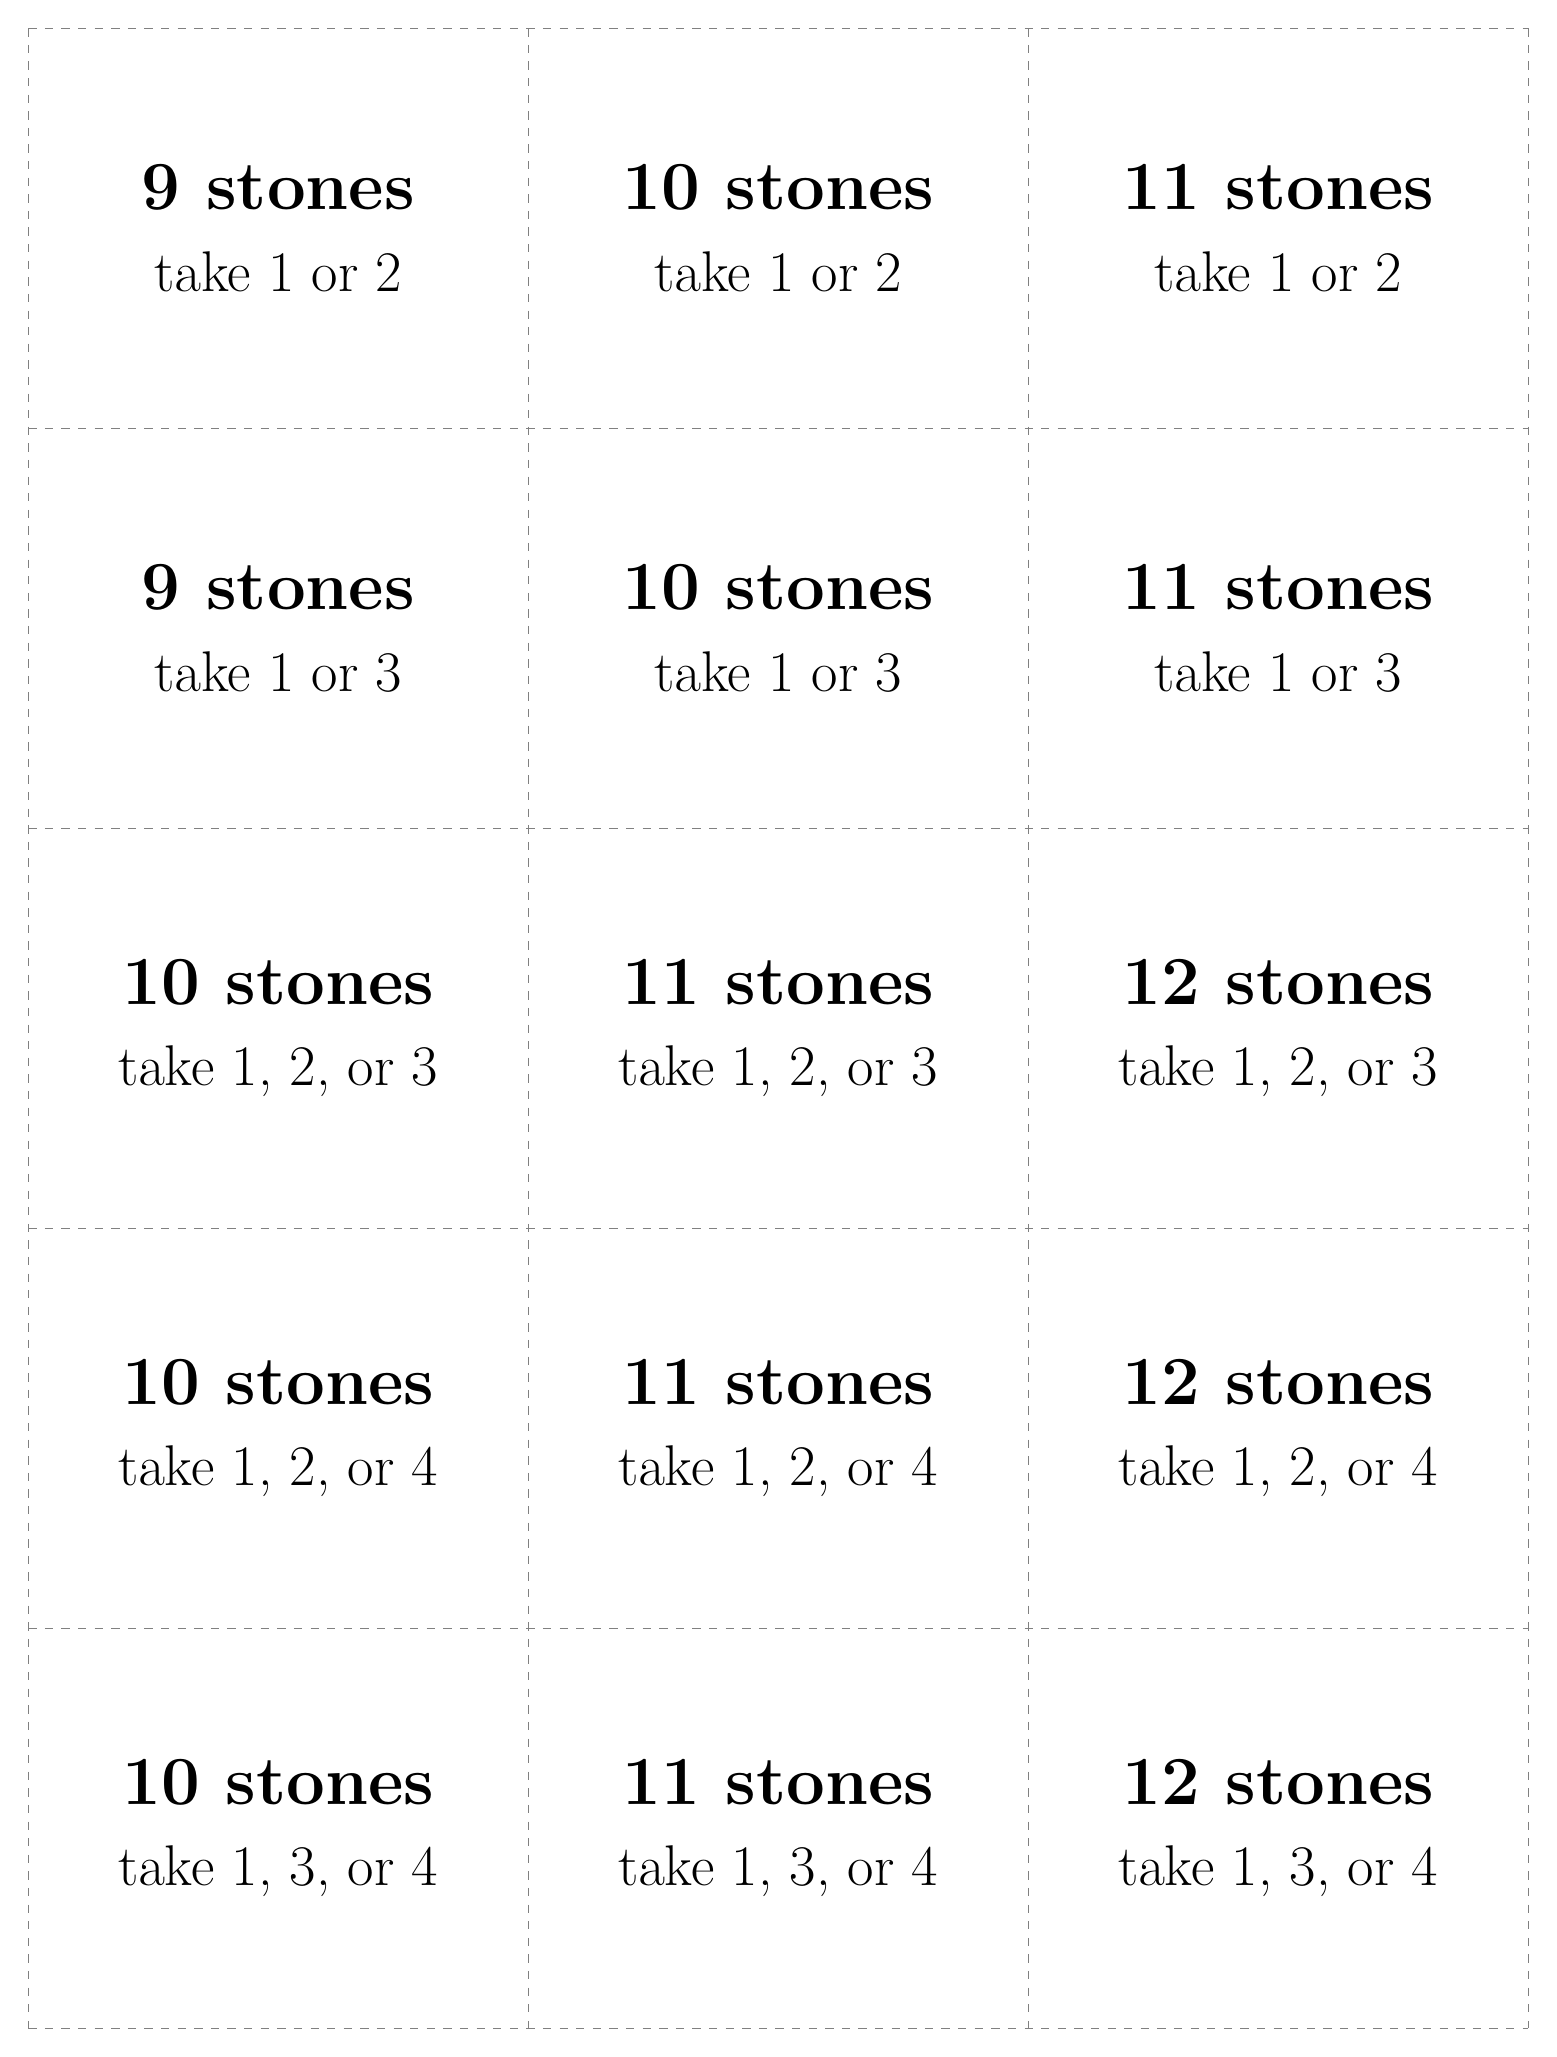
\begin{tikzpicture}
  % Cut lines
  \foreach \i in {0,...,3}
    \draw[dashed, gray] (\i*\cardwidth, 0) -- (\i*\cardwidth, -5*\cardheight);
  \foreach \j in {0,...,5}
    \draw[dashed, gray] (0, -\j*\cardheight) -- (3*\cardwidth, -\j*\cardheight);

  \card{0}{0}{9}{1 or 2}
  \card{1}{0}{10}{1 or 2}
  \card{2}{0}{11}{1 or 2}

  \card{0}{1}{9}{1 or 3}
  \card{1}{1}{10}{1 or 3}
  \card{2}{1}{11}{1 or 3}

  \card{0}{2}{10}{1, 2, or 3}
  \card{1}{2}{11}{1, 2, or 3}
  \card{2}{2}{12}{1, 2, or 3}

  \card{0}{3}{10}{1, 2, or 4}
  \card{1}{3}{11}{1, 2, or 4}
  \card{2}{3}{12}{1, 2, or 4}

  \card{0}{4}{10}{1, 3, or 4}
  \card{1}{4}{11}{1, 3, or 4}
  \card{2}{4}{12}{1, 3, or 4}
\end{tikzpicture}
\vspace*{\fill}
\end{document}
